\section{Label-Permutation Null Distributions (Supplementary)}
\label{app:perm_null}

This appendix reports the full label-shuffle permutation-null
distributions that support the ceiling and rescue claims of
Sec.~\ref{sec:results_paired}. Each permutation shuffles the
recording-level label vector before cross-validation and re-runs
the full LaBraM fine-tuning pipeline; the resulting per-run
subject-level balanced accuracy is a single draw from the null
distribution. We ran $30$ permutation seeds per dataset on the same
LaBraM recipe used for the real runs.

\paragraph{Stress cohort (contrast-bounded).} Under the canonical
LaBraM fine-tuning recipe, the real three-seed subject-level BA
($0.443 \pm 0.083$) lies inside the thirty-seed null distribution
($0.506 \pm 0.063$; null range $0.393$--$0.661$;
Fig.~\ref{fig:perm_null_density}, top). The real mean falls below
the null mean, so the one-sided test comparing real-to-null by
Mann--Whitney rank-sum is $p \geq 0.5$; the empirical $p$-floor of
$1/31 \approx 0.032$ is not approached.

\paragraph{EEGMAT cohort (anchored within-subject contrast).} Under
the matching recipe, the real three-seed BA ($0.731 \pm 0.021$)
exceeds every one of the thirty permutation-null BAs (null
$0.498 \pm 0.053$; null max $0.611$;
Fig.~\ref{fig:perm_null_density}, bottom). The real-minimum of
$0.714$ exceeds the null-maximum of $0.611$, so the one-sided
permutation $p$-value is below the $1/31 \approx 0.032$ floor.

\begin{figure}[!t]
\centering
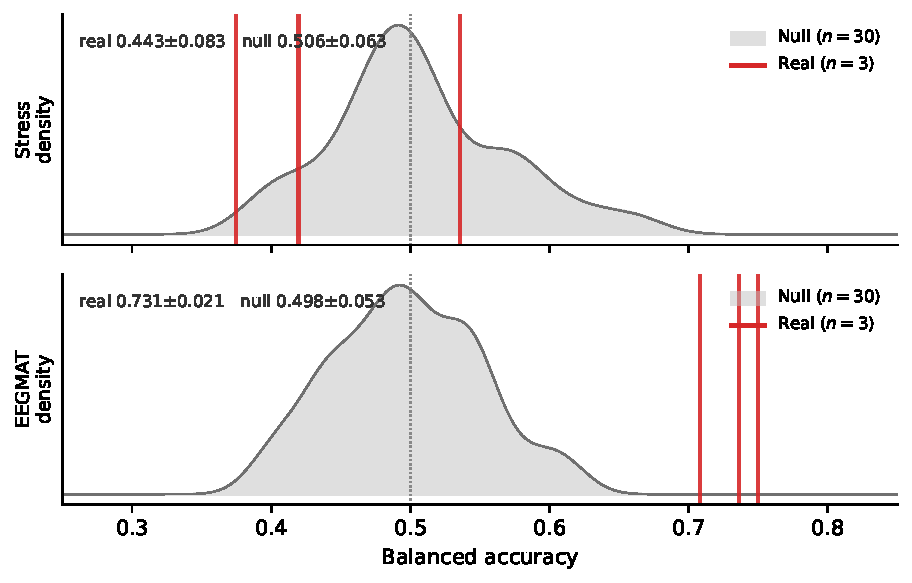
\includegraphics[width=0.9\linewidth]{figures/main/fig_perm_null_density.pdf}
\caption{Label-permutation null distributions for LaBraM
  fine-tuning on UCSD Stress (top) and EEGMAT (bottom). Grey:
  thirty-seed null kernel-density estimate. Red verticals: three real
  seeds. Dotted vertical: chance ($0.50$). The Stress real seeds sit
  inside the null distribution; the EEGMAT real seeds sit entirely
  outside it.}
\label{fig:perm_null_density}
\end{figure}

The contrast between the two panels is the representation-level
counterpart of the behavioural contrast reported in the main text:
an anchored within-subject contrast is reliably detected by
fine-tuning above chance, whereas the subject-dominated Stress
representation yields fine-tuned classification indistinguishable
from label-shuffle. Both panels use the same LaBraM recipe, the same
subject-level StratifiedGroupKFold evaluation, and the same
permutation protocol; the only difference between them is the
underlying label.
